
\clearpage{}
\section{Type directed projections}
\label{System:Projections}

In \S\ref{Intro:Update:broadcast} we discussed how references (and pointers) are used to update values within container structures, without knowledge of the surrounding container. We also discussed how they are used to update values that are shared by several different parts of the program, without needing information about how they are shared. On the other hand, in \S\ref{intro:ref-types} we saw how the use of ML style references can lead to a large amount of refactoring effort when writing programs. This is because the reference appears in the value types of terms that use them, and we must use an explicit function call to read a reference when we want the contained value.

The Disciple projection system provides a mechanism to create references on the fly, so we can use them for shared update without the need to change the structure of value types. The fact that we can provide this mechanism while still tracking enough information to perform compile type optimisations is the primary reason we have developed the type system discussed in this chapter. We also provide a separate name space associated with each type constructor, and  projection functions are placed in the name space corresponding to the type of value they project. This avoids the problem with Haskell style records, also discussed in \S\ref{Intro:Update:broadcast}, where the names of projection functions pollute the top-level scope of the program. In this thesis we restrict ourselves to associating namespaces with \emph{constructors} instead of general types. This is to avoid issues with overlapping types such as $\iList \ a$ and $\iList \ \iInt$. 

Projections are complementary to type classes. For example, when performing type inference for an expression like $\ishow \ x$, the variable $x$ may have a polymorphic type. As the instance function to use for $\ishow$ may be resolved at run time via a dictionary passing mechanism\footnote{At least it can in a mature compiler like GHC. Our prototype implementation does not yet support dictionary passing, though we are not aware of any barrier to adding it. }, the compiler itself will not know which instance function will be used. Due to this, the type of $\ishow$ in the class definition must be an upper bound of the types of all possible instances.

On the other hand, when performing type inference for the projection $x \ \odot \ \ifieldOne$, we require the type of $x$ to resolve to something that includes an outer constructor. We use this constructor to determine how to implement the projection of $\ifieldOne$. This in turn allows each of the projections named $\ifieldOne$ to return values of \emph{different} types.

% -----------------
\subsection{Default projections}
\label{System:Projections:default}

Consider the following data type definition. 

\code{
	$\kdata$ \ $\iVecTwo \ r \ a = \iVecTwo \ \{ \ x :: a; \ y :: a \ \}$
}

$x$ and $y$ are the field names of the constructor. In Haskell, this definition would introduce $x$ and $y$ as record selectors in the top level scope. In Disciple, we instead get two projections $\odot \ x$ and $\odot \ y$ that can be applied to values of type $\iVecTwo \ r \ a$, for any $r$ or $a$. As our type expressions may contain commas, we use a semicolon as a field separator instead of a comma.  Also, $\odot$ is an infix operator, and $\odot \ x$ is written \texttt{.x} in the concrete syntax. Here is an expression which uses the two projections:

\code{
	$\kdo$	
		& $\ivec$	& $= \iVecTwo \ 2.0 \ 3.0$ \\
		& $\iangle$	& $= \isqrt \ (\isquare \ \ivec \odot \ x + \isquare \ \ivec \odot \ y)$ \\
}

The projection operator $\odot$ binds more tightly than function application, so $\isquare \ \ivec \odot \ x$ should be read as $\isquare \ (\ivec \odot \ x)$. If we do not have a handy object of the required type then we can refer to the projection functions in a particular namespace directly with the $\&$ operator. For example, we could rewrite the above expression as:

\code{
	$\kdo$	& $\ivec$	& $= \iVecTwo \ 2.0 \ 3.0$ \\
		& $\iangle$	& $= \isqrt \ 		(\isquare \ (\iVecTwo\&x \ \ivec)$ \\ 	
		&		& \qq \qq \qq $ + \ 	(\isquare \ (\iVecTwo\&y \ \ivec))$ \\
}

The projections associated with field names are called \emph{default projections}. These are introduced automatically by the language definition. For $\iVecTwo$ the two projection functions are:

\code{
	$\iVecTwo \: \& \: x$	
		& $::$		& $\forall r_1 \ a. \ \iVecTwo \ r_1 \ a \lfuna{e_1} a$ \\
		& $\rhd$	& $e_1 = \iRead \ r_1$ 
	\\[1ex]
	\mc{3}{$\iVecTwo \: \& \: x \ \ (\iVecTwo \ x \ y) = x$}
	\\[3ex]
	$\iVecTwo \: \& \: y$	
		& $::$		& $\forall r_1 \ a. \ \iVecTwo \ r_1 \ a \lfuna{e_1} a$ \\
		& $\rhd$	& $e_1 = \iRead \ r_1$ 
	\\[1ex]
	\mc{3}{$\iVecTwo \: \& \: y \ \ (\iVecTwo \ x \ y) = y$}
}

This syntax is similar to the use of $::$ in C++ to define class methods. For example, the name of a method in a class named $\iVecTwo$ would be $\iVecTwo::x$. 

\clearpage{}
% ---------------------------
\subsection{Ambiguous projections and type signatures}
\label{System:Projections:ambiguous}

Ambiguous projections arise when we project a value whose type is not constrained to include an outer constructor. For example, the projections in the following code are ambiguous:

\code{
	$\itupleOfVec$ = $\lambda \ivec. \ (\ivec \ \odot \ x, \ \ivec \ \odot \ y)$ 
}

Without further information, the type of $\ivec$ in this code is just a variable. If our program included more than one data type that had an $x$ or $y$ field, then there would be no way of knowing which projection function to use. 

The programmer can resolve this problem by providing a type signature that constrains the type of $\ivec$. For example:

\code{
	\mc{2}{$\itupleOfVec :: \iVecTwo a \to (a, \ a)$} \\
	$\itupleOfVec$ = $\lambda \ivec. \ (\ivec \ \odot \ x, \ \ivec \ \odot \ y)$ 
}

Note that we do not need to provide region, effect or closure information in type signatures. The fact that this information is missing from the above signature can be determined from the kind of $\iVecTwo$, and it can be filled in by the type inference process. 

% ---------------------------
\subsection{Pull back projections}
\label{System:Projections:pull-back}

Pull back projections allow the programmer to create references to the fields of a record. For example, a reference to the $x$ field of our $\iVecTwo$ type can be created with $\ivec \: \odot_{\#} \: x$, pronounced ``$\ivec$ pull $x$''. If the type of $\ivec$ is $\iVecTwo \ r_1 \ a$ then the type of $\ivec \: \odot_{\#} \: x$ is $\iRef \ r_1 \ a$. If we imagine $\iRef$ types being equivalent to pointers in C, then $\ivec \: \odot_{\#} \: x$ has the same meaning as the C expression \texttt{\&(vec.x)}. The $:=_{\#}$ function (pronounced ``update ref'') is then used to update the value of the field. Note that $\ivec \: \odot_{\#} \: x$ and $:=_{\#}$ are written as \texttt{vec\#x} and \texttt{\#=} in the concrete syntax.

Here is the type of $:=_{\#}$

\code{
	$(:=_{\#})$  
		& $::$		& $\forall r_1 \ a. \ \iRef \ r_1 \ a \lfun a \lfuna{e_1 \ c_1} ()$ \\
		& $\rhd$ 	& $e_1 = \iWrite \ r_1$  \\
		& \ ,		& $c_1 = x : \iRef \ r_1$ \\
		& \ ,		& \mc{2}{$\iMutable \ r_1$}
}

Here is an example that creates a vector then updates one of its components:

\code{
	$\kdo$	& $\ivec$	& $= \iVecTwo \ 2.0 \ 3.0$ \\
		& $\iref$	& $= \ivec \: \odot_{\#} \: x$ \\
		& \dots \\
		& $\iref$	& $:=_{\#} \ 5.0$ \\
		& \dots \\
}

After the update statement has been executed, the projection $\ivec \ \odot \ x$ will return the value $5.0$ instead of $2.0$. Pull back projection functions can also be accessed directly. Here are the names and types of the pull back projections for the $x$ and $y$ fields:

\code{
	$\iVecTwo \: \& \:x_{\ipull}$	
		& $ :: \forall r_1 \ a. \ \iVecTwo \ r_1 \ a \fun \iRef \ r_1 \ a$  
	\\[1ex]
	$\iVecTwo \: \& \:y_{\ipull}$
		& $ :: \forall r_1 \ a. \ \iVecTwo \ r_1 \ a \fun \iRef \ r_1 \ a$ 
}

Note that the created reference shares the same region variable as the projected value. Also note that as $\iVecTwo$ only has a single data constructor, the functions $x_{\ipull}$ and $y_{\ipull}$ are pure. This is because when we evaluate an expression like $\ivec \: \odot_{\#} \: x$, we do not need to access the $\ivec$ object at all. We simply allocate a new reference that contains a pointer into it. This can be done based on the address of the $\ivec$ object, the object itself is not needed. For example, if we say:

\code{
	$\ivec$ 	& $:: \iVecTwo \ r_1 \ (\iFloat \ r_2) \ (\iFloat \ r_3)$  \\
	$\ivec$		& $= \iVecTwo \ 2.0 \ 3.0$
}

then we would have:

\code{
	$\iref$	& $:: \iRef \ r_1 \ (\iFloat \ r_2)$ \\
	$\iref$ & $= \ivec \: \odot_{\#} \: x$
}

which produces the following objects in the store:

\begin{center}
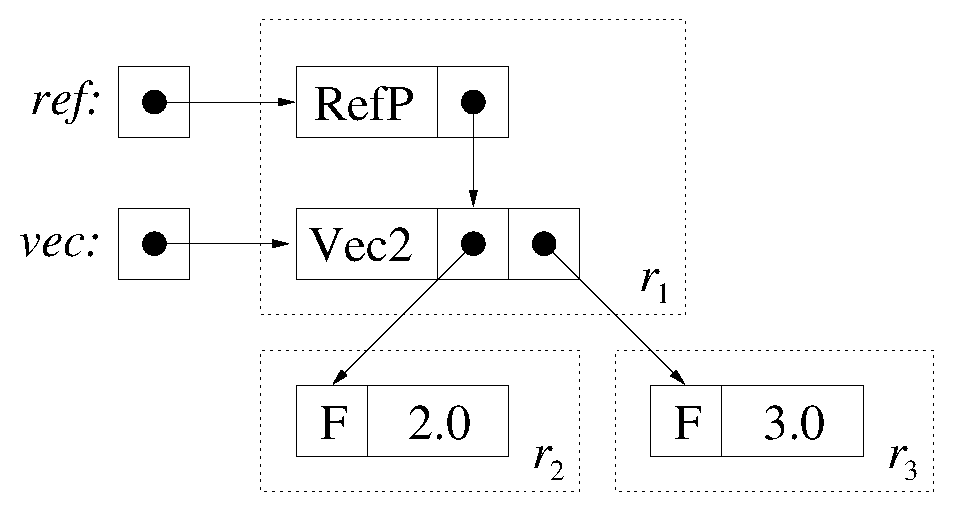
\includegraphics[scale=0.5]{2-System/fig/projections/pull-back}
\end{center}

We use the tag $\iRefP$ to record the fact that the $\iref$ object is a pull back reference that points into another object, as opposed to a regular ML style reference. When we execute the statement $\iref :=_{\#} 5.0$, it is the pointer inside the $\ivec$ object that is updated, not the $\iFloat$ object itself:

\begin{center}
\includegraphics[scale=0.5]{2-System/fig/projections/pull-back-update}
\end{center}

This leaves the old $2.0$ object to be reclaimed by the garbage collector.

The benefit of this system over ML style references is that we are able to update data structures without needing $\iRef$ in their type definitions, which addresses the refactoring problem discussed in \S\ref{intro:ref-types}. Note that in the above diagram, both the $\iVecTwo$ and $\iRefP$ objects are in the same region, $r_1$. This means that when we use a function like $(:=_{\#})$ to update the vector via the reference, the vector object will also be marked as mutable.

Although we don't \emph{need} ML style references, Disciple does support them, and we can equally define:

\code{
	$\kdata$ \ $\iVecTwo \ r_1 \ a = \iVecTwo \ \{ \ x :: \iRef \ r_1 \ a; \ y :: \iRef \ r_1 \ a \ \}$
}

In this case we would construct a vector with:

\code{
	$\ivec$		& $:: \iVecTwo \ r_1 \ (\iFloat \ r_2) \ (\iFloat \ r_3)$ \\
	$\ivec$		& $= \iVecTwo \ (\iRef \ 2.0) \ (\iRef \ 3.0)$
}

This produces the following objects in the store:

\begin{center}
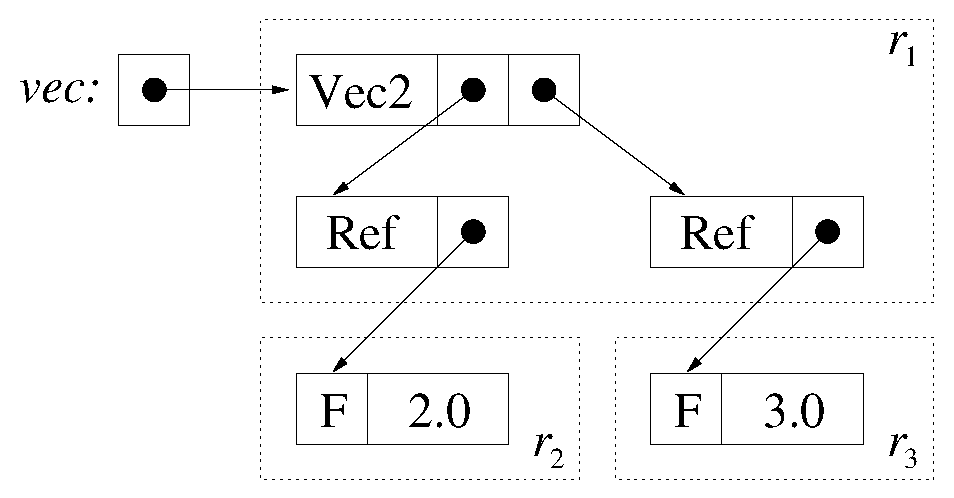
\includegraphics[scale=0.5]{2-System/fig/projections/vec-ref}
\end{center}

Here, the reference objects include the constructor tag $\iRef$, instead of $\iRefP$ as before. This indicates that to update these references, the pointer in the object itself should be modified, not the word that is pointed to.




\subsection{Custom projections}
\label{System:Projections:custom}

Along with the default field projections introduced by data type declarations, the programmer can also define their own custom projection functions. In fact, any variables they desire can be added to the name space associated with a type constructor, whether they are bound to functions that perform true projections, or not. For example, we can add a $\imagnitude$ function to the $\iVecTwo$ name space with:

\code{
	\mc{2}{$\kproject \ \iVecTwo \ \kwhere$} \\
		& $\imagnitude \ (\iVecTwo \ x \ y)$ \\
		& \qq $= \isqrt \ (\isquare \ x + \isquare \ y)$
}

We use $\odot \: \imagnitude$ to invoke this new projection. For example:

\code{
	$\kdo$	& $\ivec$	& $= \iVecTwo \ 2.0 \ 3.0$ \\
		& $\iputStr$	& $($``\texttt{The magnitude is:}" ++ $(\ishow \ \ivec \odot \imagnitude))$
}

Unlike default projections, custom projections can be defined to take extra arguments. For example, here is a projection to determine the dot product of two vectors:

\code{
	\mc{2}{$\kproject \ \iVecTwo \ \kwhere$} \\
		& $\idot \ (\iVecTwo \ \ixOne \ \iyOne) \ (\iVecTwo \ \ixTwo \ \iyTwo)$ \\
		& \qq $= \ixOne * \ixTwo + \iyOne * \iyTwo$
}

We can then use it as:

\code{
	$\kdo$	& $\ivec$	& $= \iVecTwo \ 2.0 \ 3.0$ \\
		& $\ivecTwo$	& $= \iVecTwo \ 4.0 \ 5.0$ \\
		& $\iputStr$	& $($``\texttt{The product is:}" ++ $(\ishow \ \ivec \ \odot \idot \ \ivecTwo))$
}

This allows a style of programming similar to using local methods in object oriented languages. For example, in Java we would write \texttt{vec.dot(vec2)}. With Disciple code, we find it helpful to view the projection $\odot \idot$ as a single operator. This highlights the similarities with the equivalent expression in vector calculus, $\ov{v_1} \bullet \ov{v_2}$.

Disciple also provides a punning syntax for adding variables to projection namespaces. This allows the programmer to add variables defined elsewhere in the module, and helps reduce the level of indenting in the code. For example, we could define our $\imagnitude$ and $\idot$ projections with:

\code{
	\mc{2}{$\kproject \ \iVecTwo \ \kwith \ \{ \imagnitude, \idot \}$} 
	\\[1em]
	$\imagnitude \ (\iVecTwo \ x \ y)$ \\
	\qq $= \isqrt \ (\isquare \ x + \isquare \ y)$ 
	\\[1em]
	$\idot \ (\iVecTwo \ \ixOne \ \iyOne) \ (\iVecTwo \ \ixTwo \ \iyTwo)$ \\
	\qq $= \ixOne * \ixTwo + \iyOne * \iyTwo$
}

We find this syntax useful when writing library code. Our usual approach is to define all the ``helper'' functions for a particular data type in the same module that declares it. These helper functions are present in the top level scope of the module, but are not exported from it directly. We use the punning syntax to add the helper functions to the projection namespace for the data type. We then export the data type name, and the projection namespace along with it. This allows us to write the majority of our program in the familiar Haskell style, while reducing the opportunity for name clashes between modules.
	
